\begin{center}
{\textbf{Mardi 17 août 2021 : Premiers cours}}
\end{center}
\vspace{2mm}

8h. Certains élèves particulièrement impatients se penchent déjà sur les exos de la muraille.

9h. Le groupe A découvre les bases du raisonnement mathématiques avec Jérémy, tandis que les élèves du groupe B sont initiés à la chasse aux angles par Domitille. Dans le groupe C, les stagiaires se familiarisent avec le double-comptage avec Arthur. Aurélien et Théodore font travailler leurs élèves du groupe D sur des problèmes d’arithmétique et combinatoire.

\begin{figure}[H]
\centering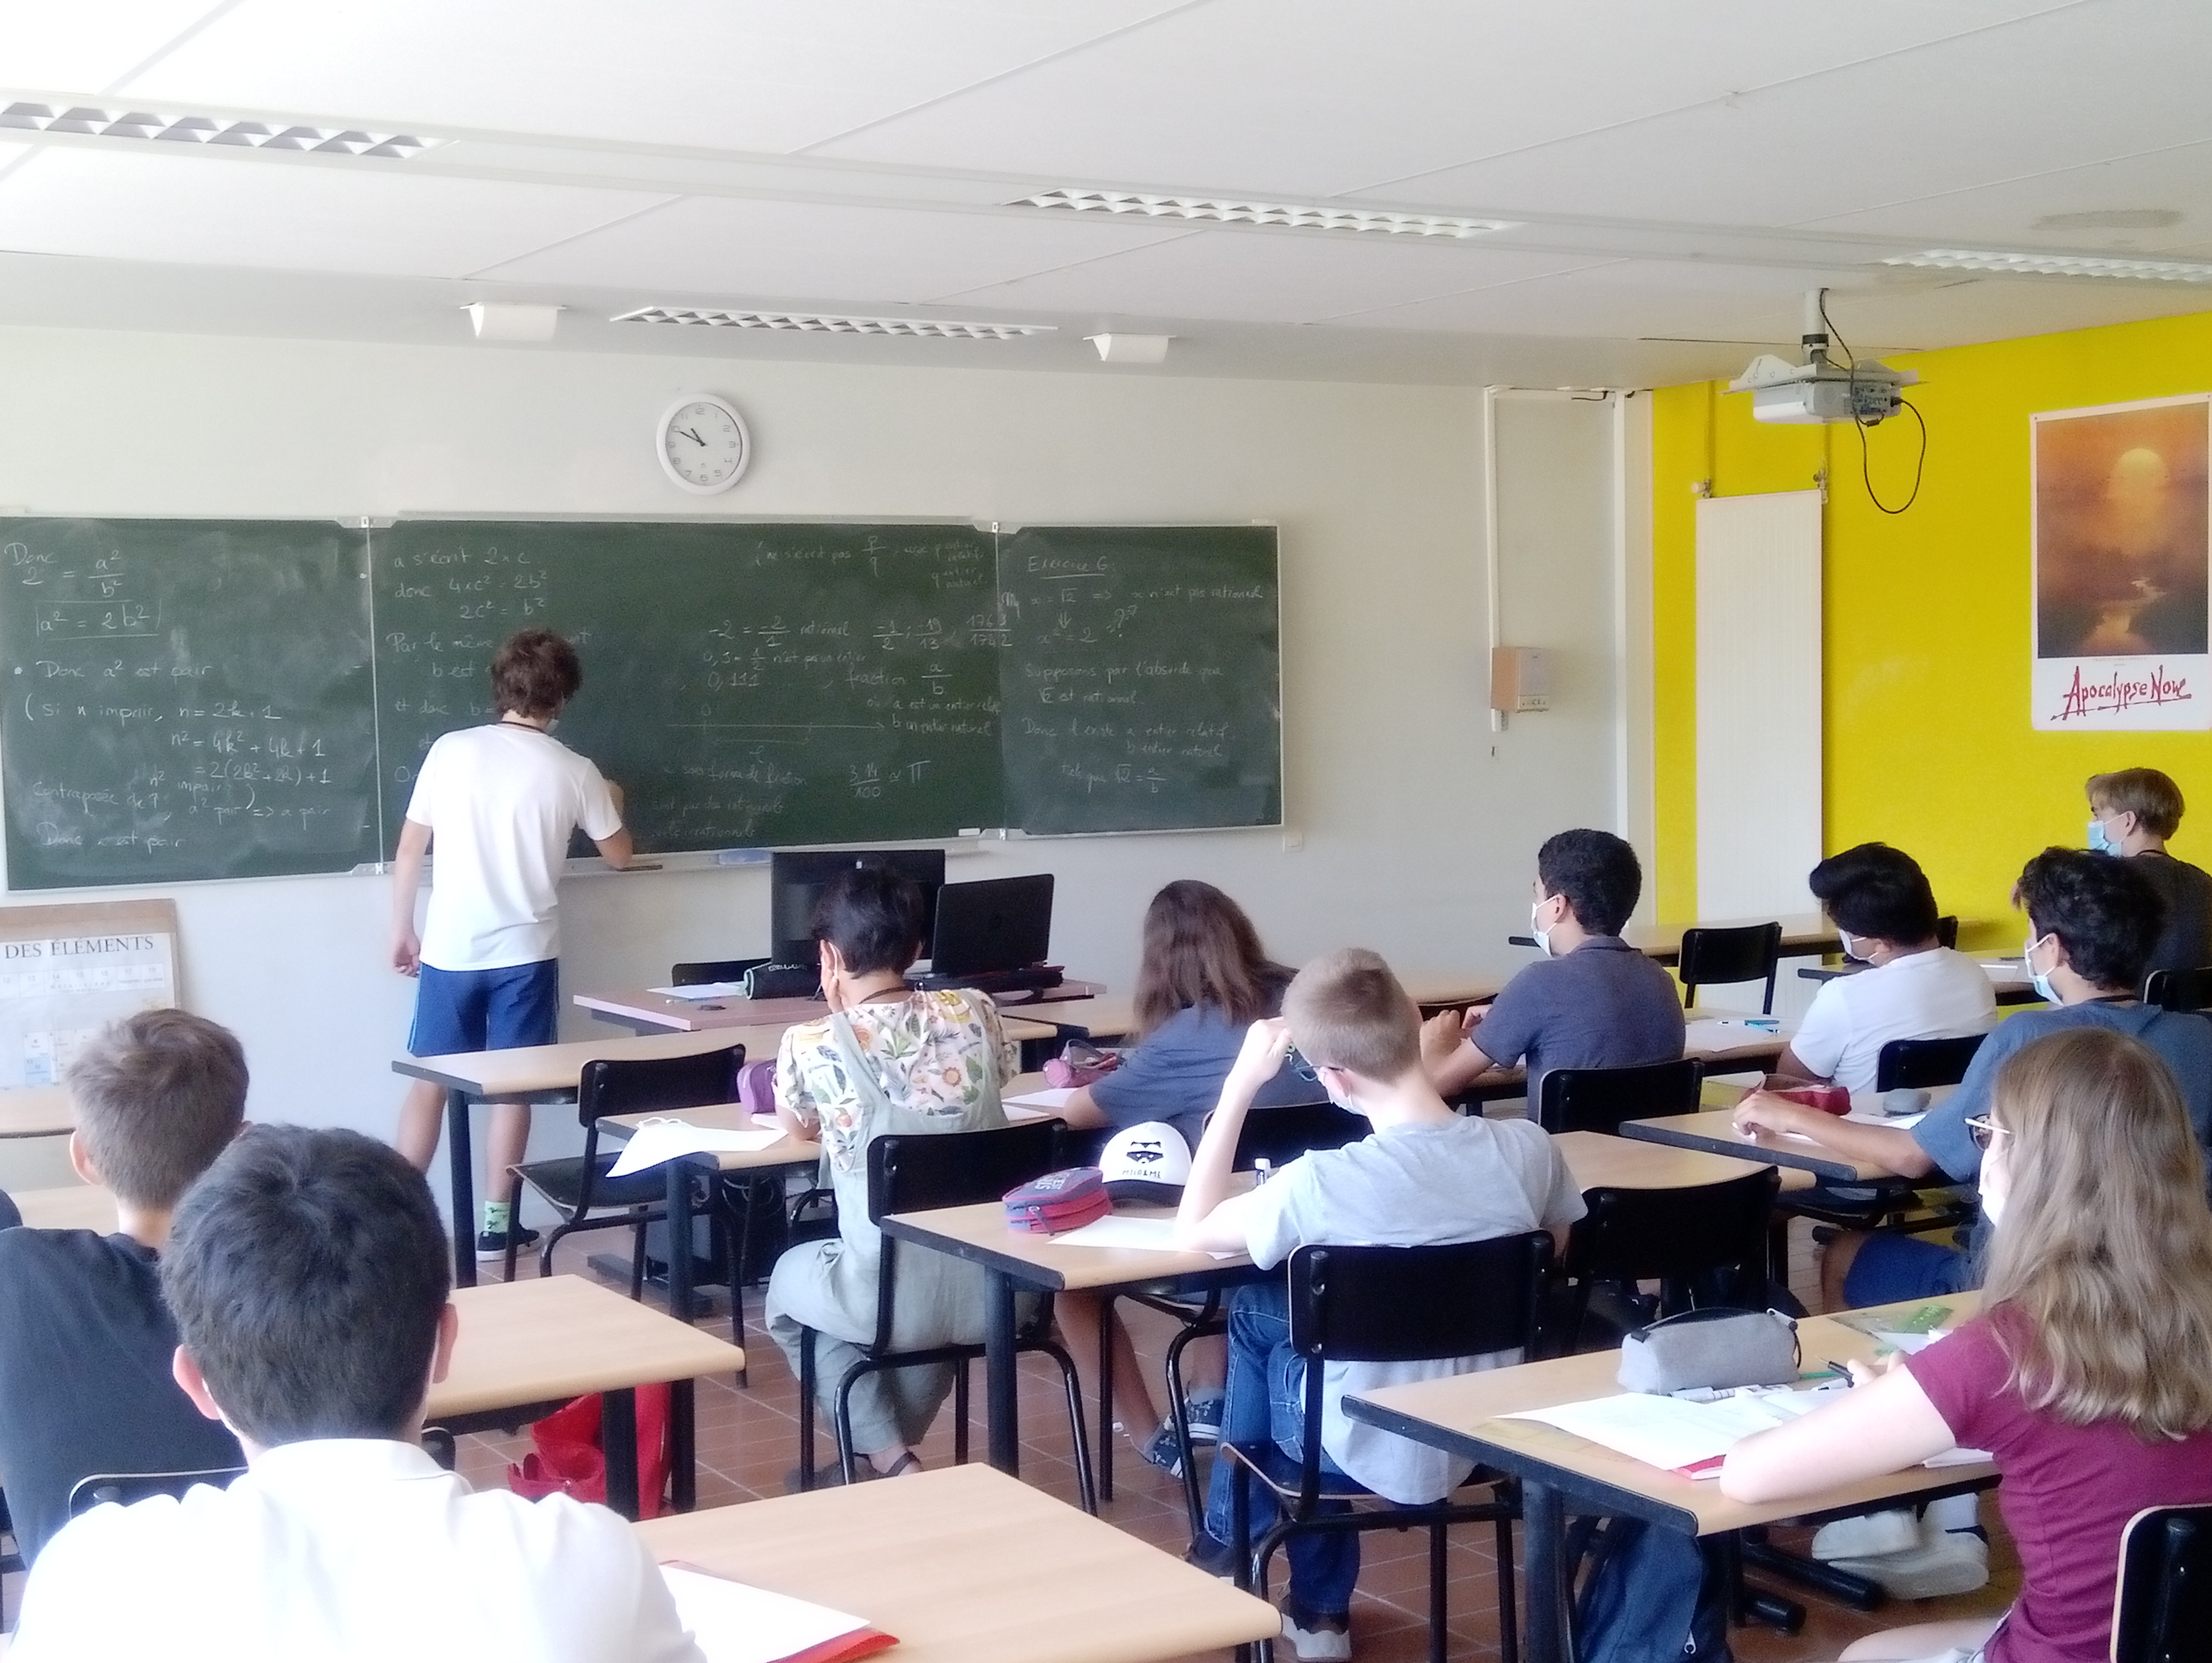
\includegraphics[width=6cm]{CR-17-0.jpg}\hspace{2cm}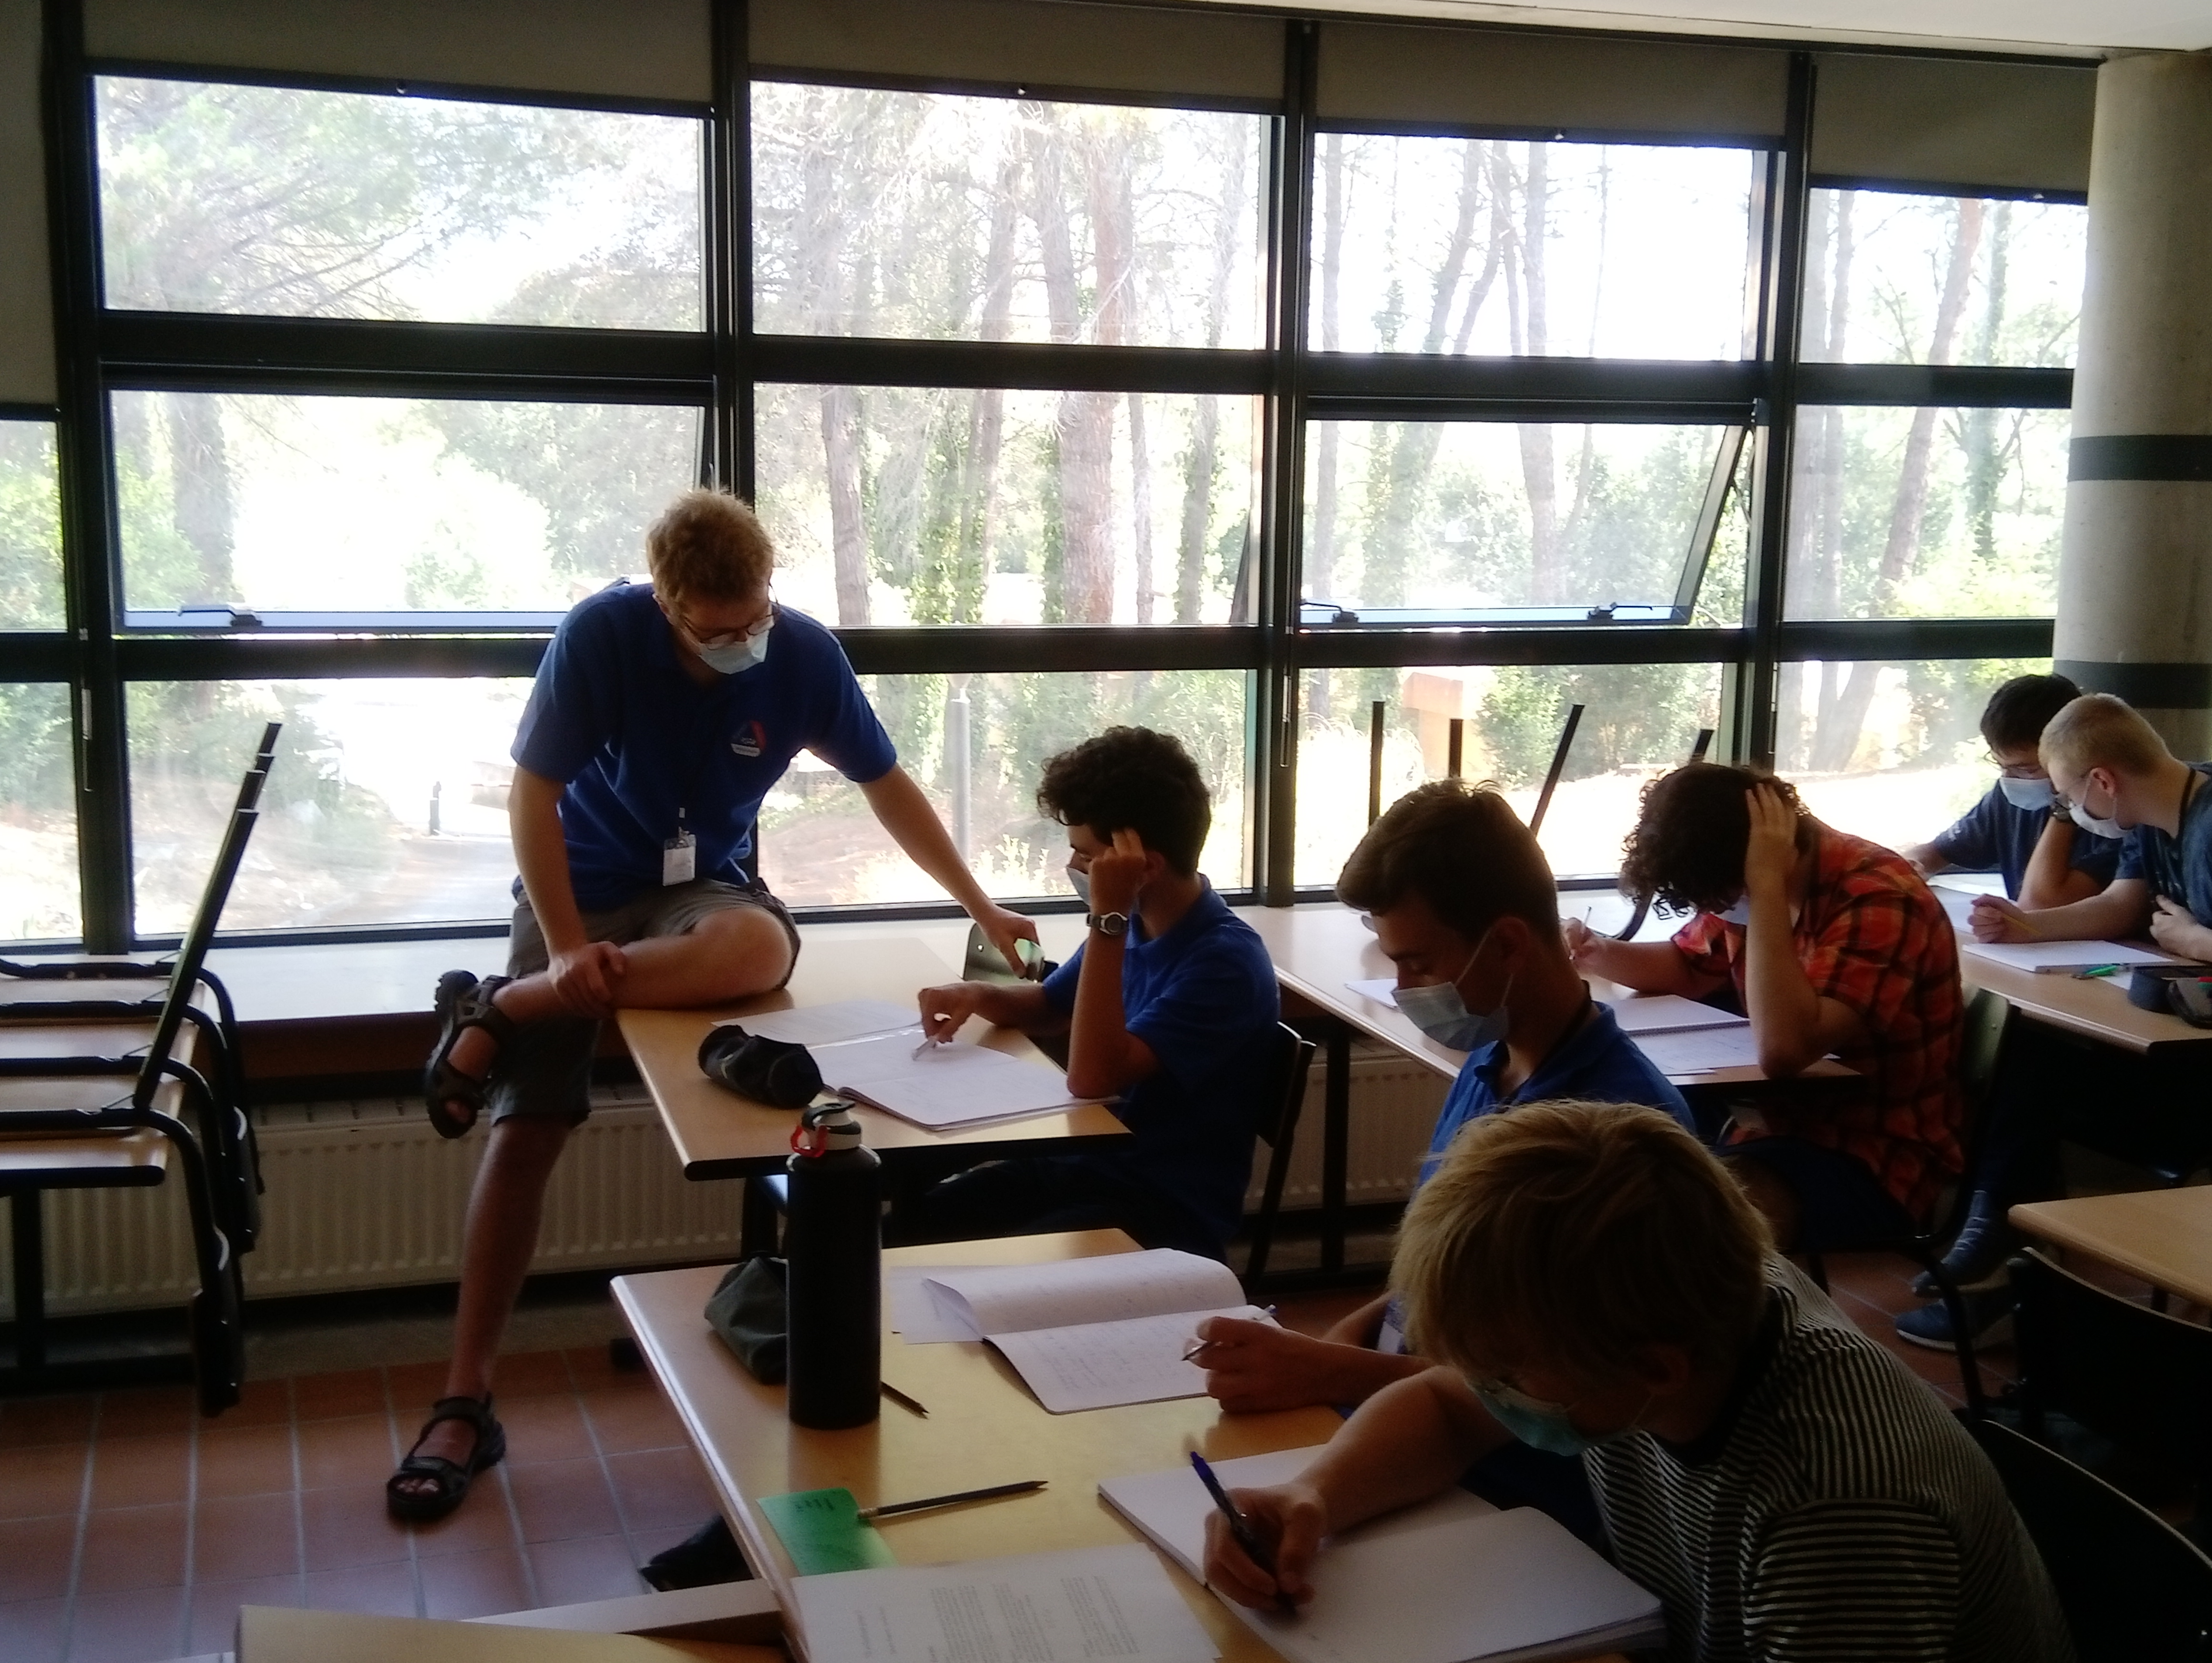
\includegraphics[width=6cm]{CR-17-1.jpg}
\caption{Découverte des mathématiques avec Jérémy dans le groupe A, tandis que Le groupe D réfléchit intensément.}
\end{figure}

13 h 30. L’après-midi, c’est au tour du groupe A de faire connaissance de la chasse aux angles avec Alexander. Le groupe B, pendant ce temps, découvre (ou redécouvre) la récurrence avec Matthieu. Dans les groupes plus avancés on fait de l’algèbre et arithmétique : un TD sur les polynômes chez Tristan, le (petit) théorème de Fermat et l’ordre modulaire chez Victor.

Une fois les cours terminés, c’est l’heure de se changer les idées!

Une bonne trentaine de stagiaires bravent le soleil brûlant pour jouer du volley-ball ou du foot. (Eh oui, contrairement aux préjugés, des matheux qui font du sport, ce n’est pas de la science-fiction…) Heureusement, malgré les conditions thermiques extrêmes, les cours de secourisme livrés par Pierre-Marie aux nouveaux recrus d’Animath ne seront pas requis.

\begin{figure}[H]
\centering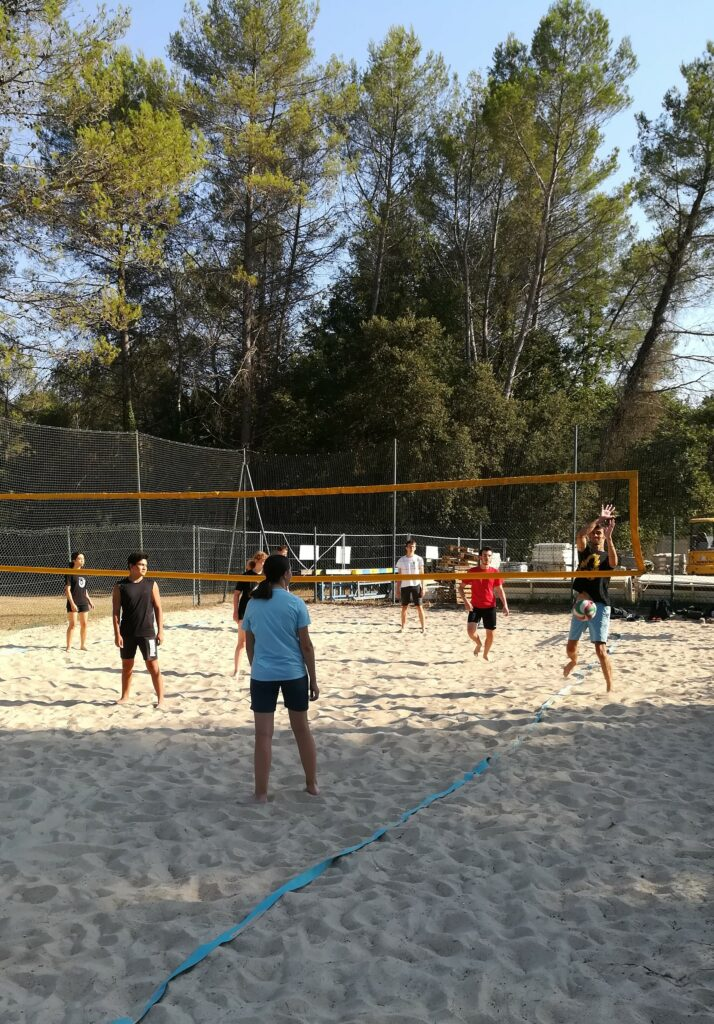
\includegraphics[width=6cm]{CR-17-2.jpg}
\caption{Premiers matchs de volley}
\end{figure}

Pendant ce temps, un autre groupe d’élèves encadrés par Théodore et Arthur part en promenade vers le magasin des alentours pour faire le plein de provisions : car il est bien connu que les mathématiques génèrent des pertes énergétiques qu’aucune cantine ne peut compenser.

20h. À l’heure de la conférence, c’est Victor qui s’empare de la scène. Le présentateur explique comment faire tenir des tours de briques parallélépipédiques, de sorte qu’elle dépasse le bord de la table. Il est assisté de Pierre-Marie et Matthieu, qui illustrent ses propos avec l’aide de 108 paquets de cartes.


\begin{figure}[H]
\centering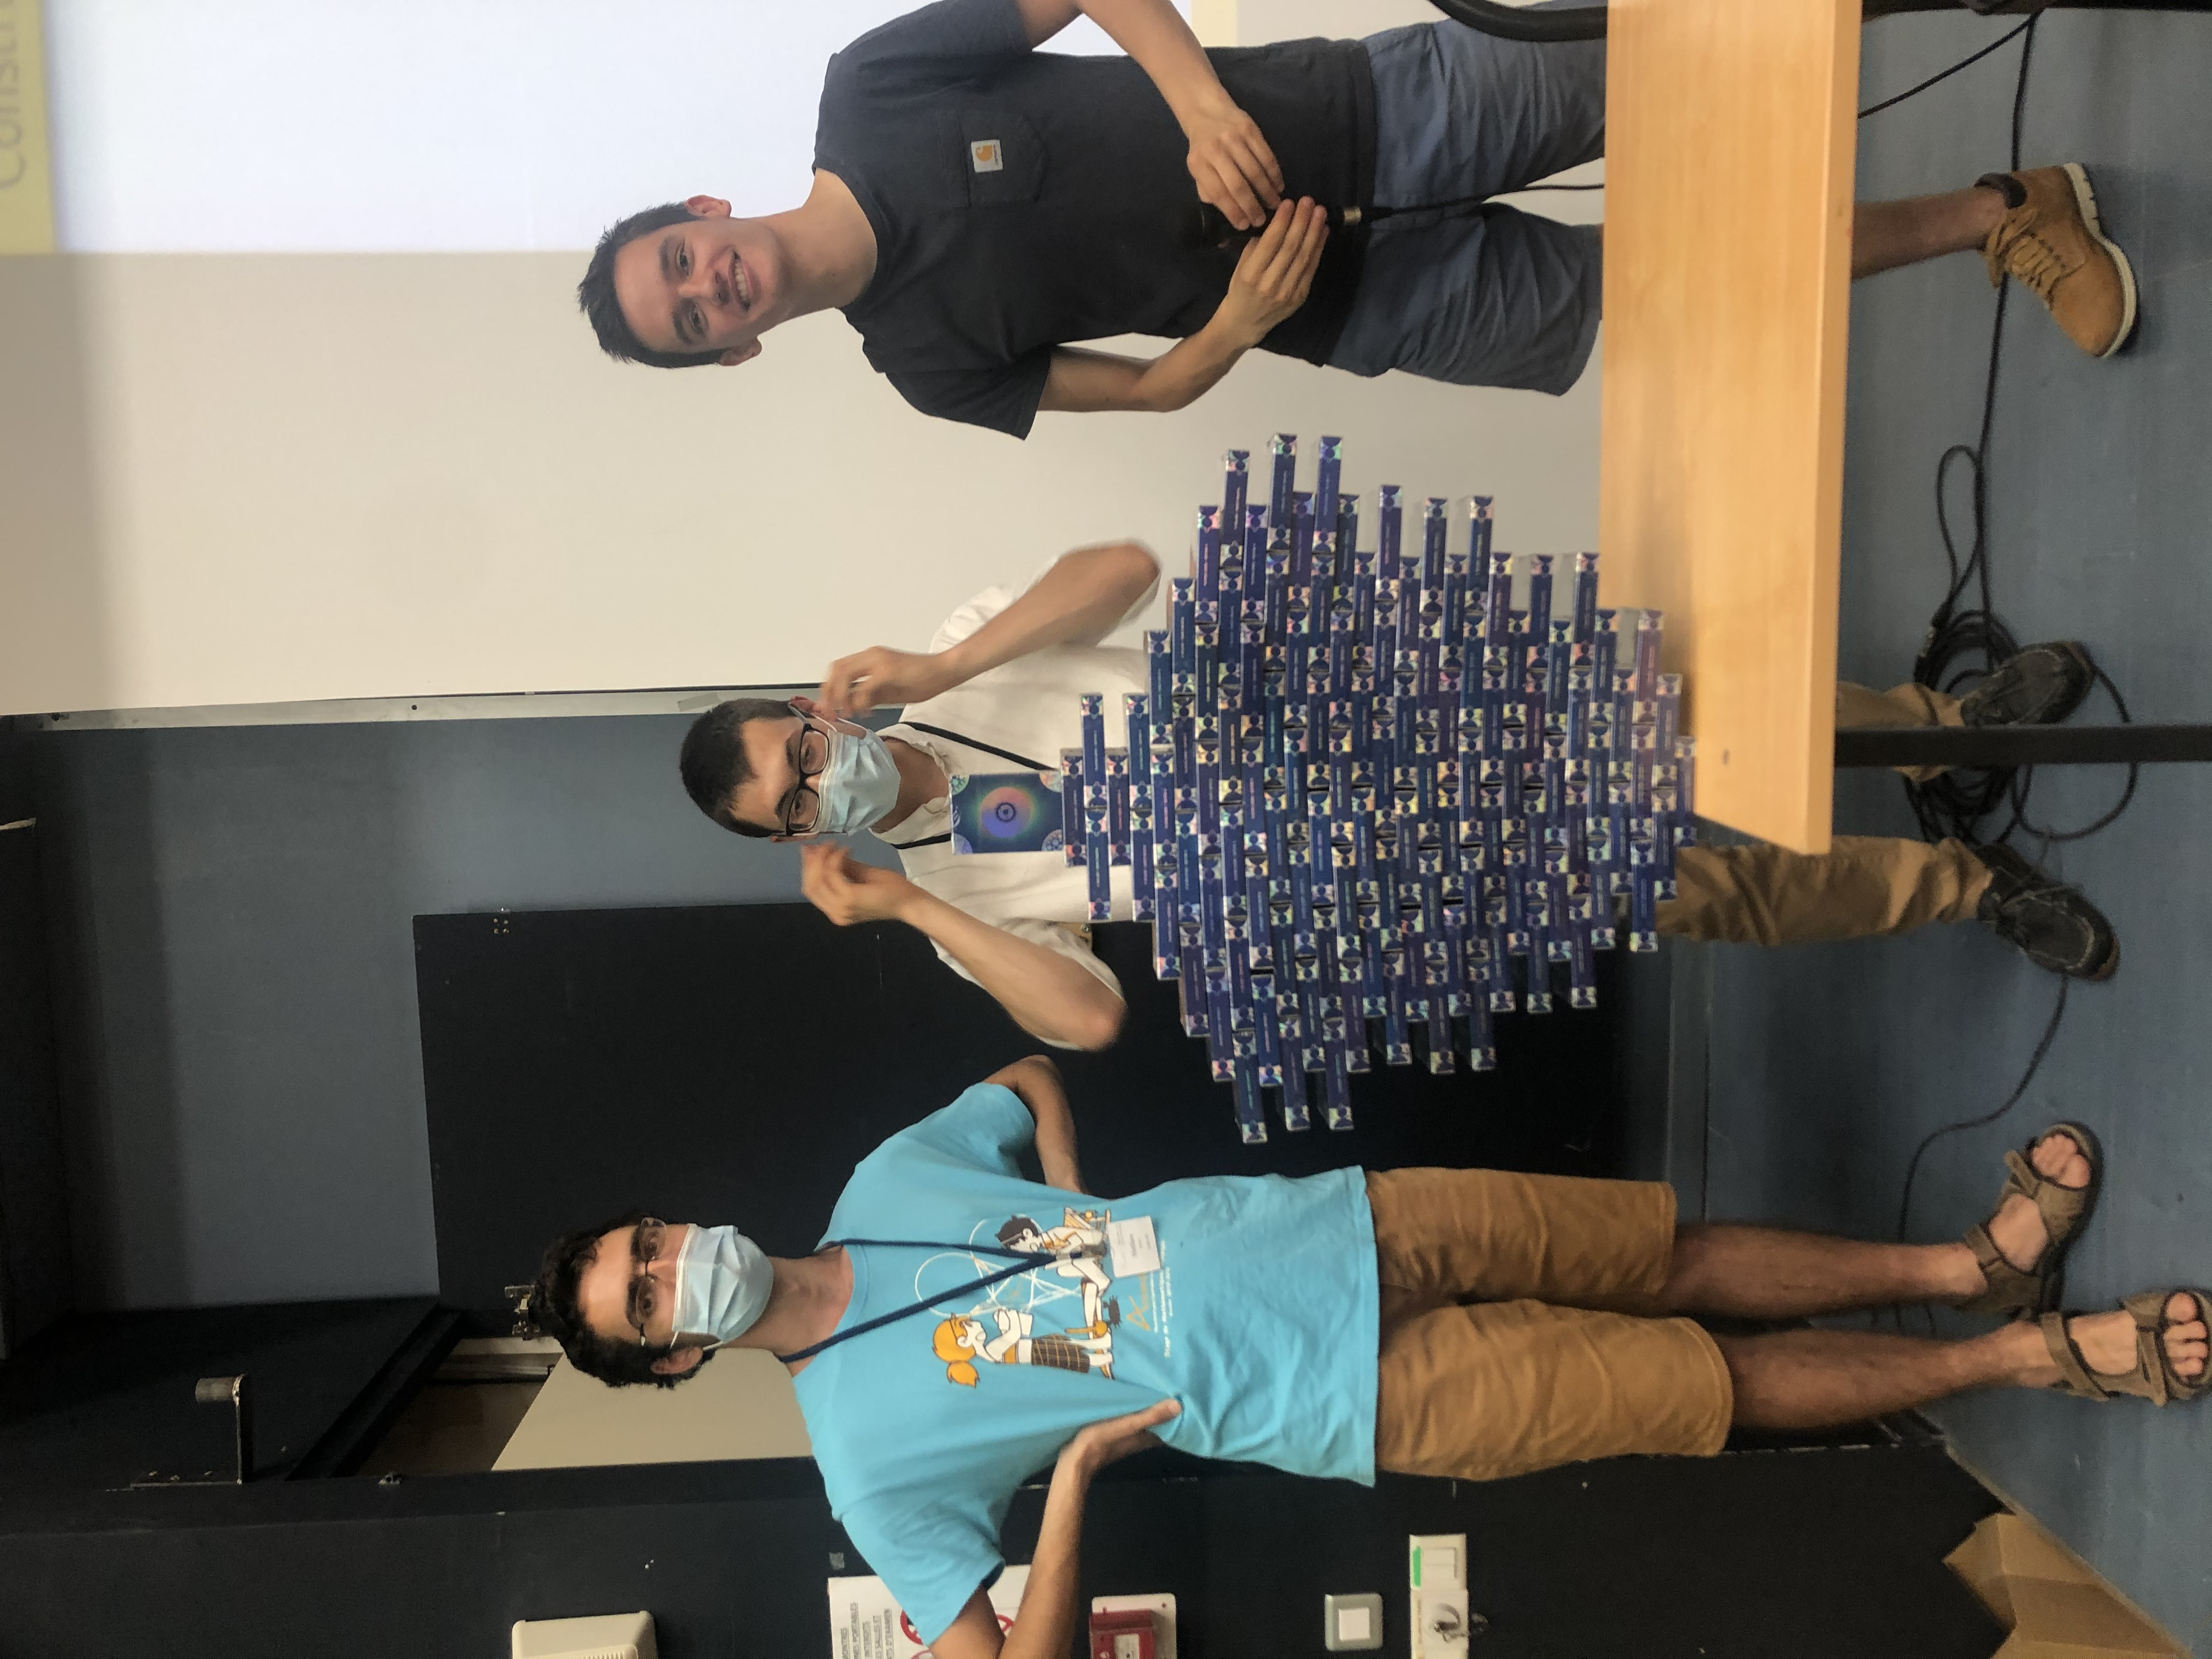
\includegraphics[height=7cm]{CR-17-3.jpg}\hspace{2cm}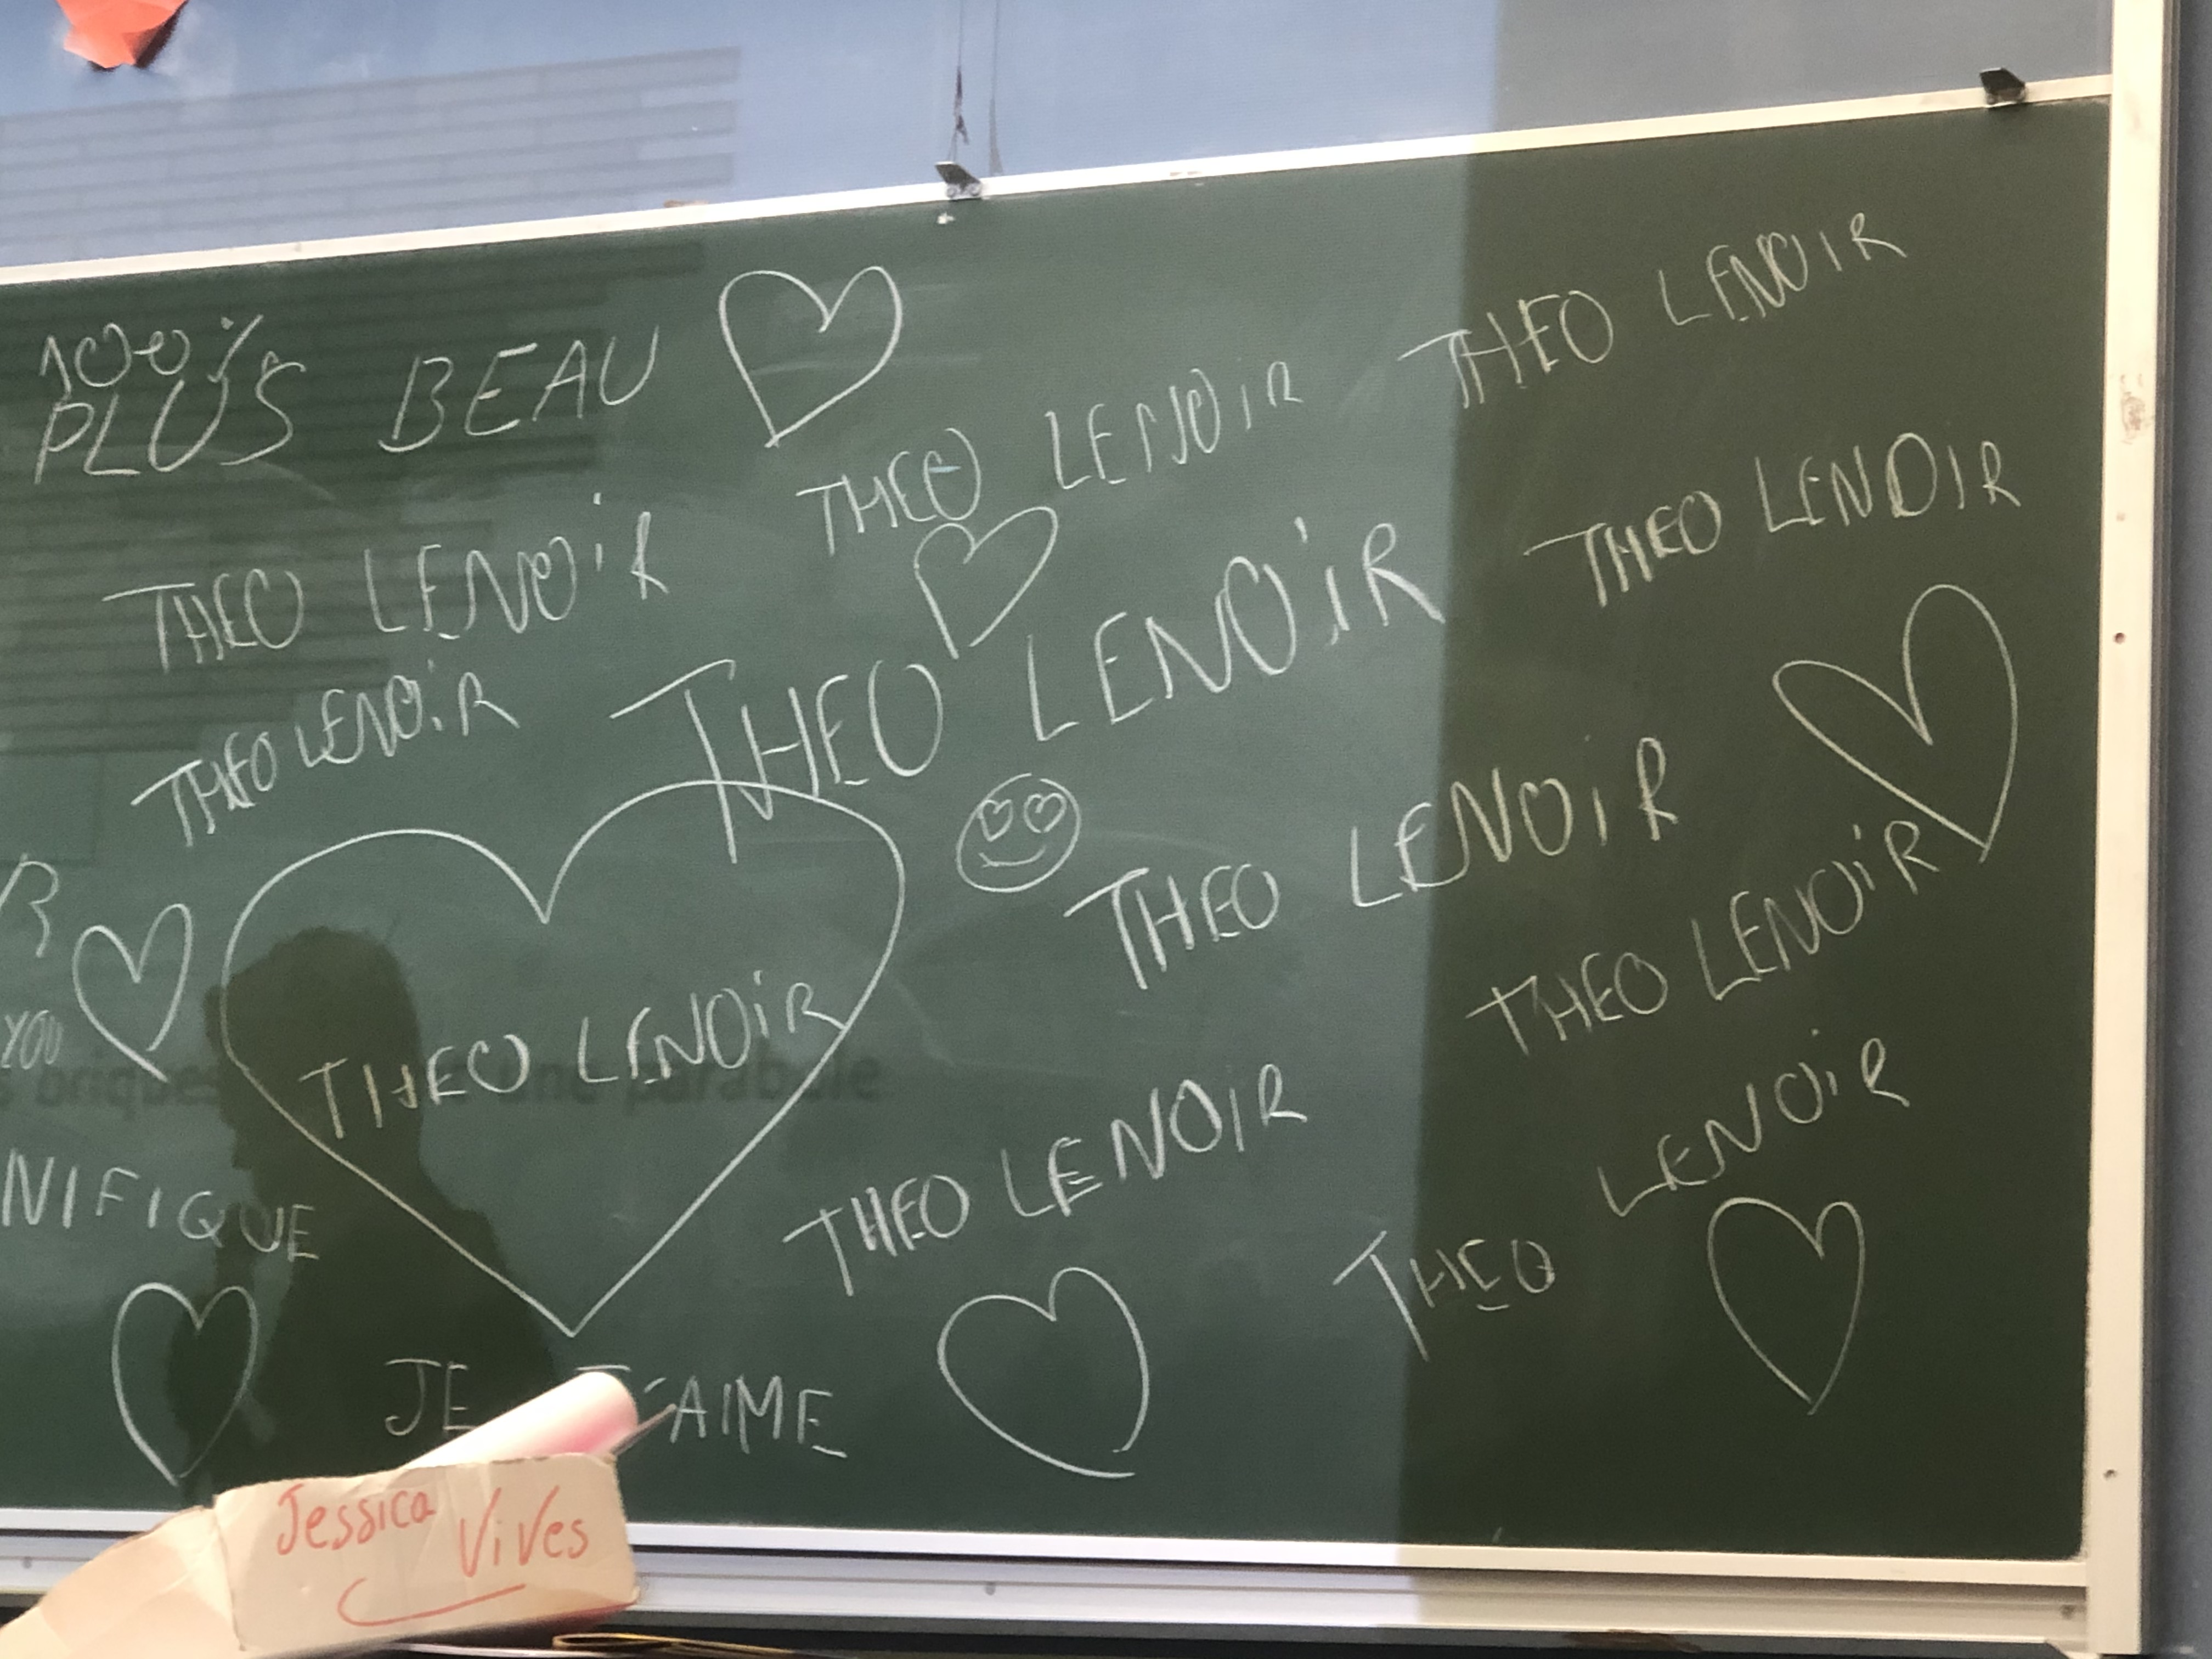
\includegraphics[height=7cm]{CR-17-4.jpg}
\caption{Le tout s’achève par une démonstration grandeur nature. Un certain animatheur semble s'être constitué un fanclub.}
\end{figure}

21h. Première soirée astronomie du stage.